\documentclass[landscape,12pt,openany]{book}

\usepackage{multicol}
\usepackage{graphicx}
\graphicspath{{./images/}}
\usepackage[margin=.5in, paperwidth=9in, paperheight=7in]{geometry}
\usepackage{titlesec}
\usepackage{xfrac}
\usepackage{framed}
\usepackage{gensymb}
\usepackage[abs]{overpic}
\setlength\unitlength{1in}
\usepackage{color}

\usepackage{cookbook}  % custom style

\titlespacing*{\chapter}{0em}{-3em}{1em}
\titleformat{\chapter}{\normalfont\huge\bfseries}{\chaptertitlename\
\thechapter:}{20pt}{\Huge}
\renewcommand{\thesection}{}  % don't show the section numbers
\titleformat{\section}[block]{\titlerule\scshape\large\filcenter\vspace{2pt}}{}{0em}{}[\titlerule]
\titleformat{\subsection}[block]{\scshape\large\filcenter}{}{0em}{}[\titlerule]
\setlength{\parindent}{1em}
\setlength{\columnseprule}{0.4pt}
\pagestyle{plain}
\raggedbottom
\usepackage[utf8]{inputenc}
\usepackage[T1]{fontenc}

\begin{document}

\rmfamily

\begin{titlepage}
    \newgeometry{margin=0in,hmargin=-12pt}
    \begin{overpic}[height=\paperheight,tics=1]{cover.jpg}
        \put(6,6){\Huge\bf\color{white} Cookbook 2013}
        \put(6.85,5.5){\Large\bf\color{white} Chase Seibert}
    \end{overpic}
    \restoregeometry
\end{titlepage}

\columnsep=2em
\setlength{\columnseprule}{0pt}.

\setcounter{page}{0}
\cleardoublepage
\setcounter{tocdepth}{1}
\tableofcontents

\chapter{Salads}
\section{Caesar Salad}
\begin{recipe}

Place serving bowls and large mixing bowl in the freezer.

\ingredients{
    \sfrac{1}{2} & loaf rye bread \\
    \sfrac{1}{4} & cup olive oil \\
              5  & garlic cloves \\
}

Simmer smashed garlic cloves in oil for 10 minutes to flavor the oil.

Cut bread into \sfrac{1}{2} inch cubes. Spread on a baking sheet and paint with olive oil mixture.

Bake at 350\degree{} for 10 minutes, and then continue to bake, watching closely, until golden brown.

Place croûtons in an open container and put in the freezer for 10 minutes.

\ingredients{
   1 & block parmesan reggiano \\
}

Grate 1 cup coarse, and \sfrac{1}{2} cup fine.

\ingredients{
    2 & heads romaine hearts \\
}

Cut into \sfrac{3}{4} inch rounds, separate and then chop roughly.

\ingredientsLeft{
    & dressing \\
    & fresh pepper \\
}

When you're ready to serve, remove large mixing bowl from freezer. Combine lettuce, cheese, pepper and two large spoonfuls of dressing.

Add croûtons, and mix again briefly. Turn out into serving bowls from the freezer.

\subsection{Caesar Dressing}

\ingredients{
               1 & large egg \\
               3 & tablespoons lemon juice \\
               1 & teaspoon Worcestershire \\
   1\sfrac{1}{2} & teaspoon anchovy paste \\
               1 &  clove garlic \\
}

Blanch egg in shell for 45 seconds in boiling water. Remove and crack into a small bowl. Whisk with other ingredients.

\ingredients{
    \sfrac{1}{3} & cup olive oil (extra-virgin) \\
}

Slowly whisk oil into the dressing. Season to taste with salt and pepper.

\end{recipe}

\newgeometry{margin=0in}
\begin{figure}[p]
    \centering
    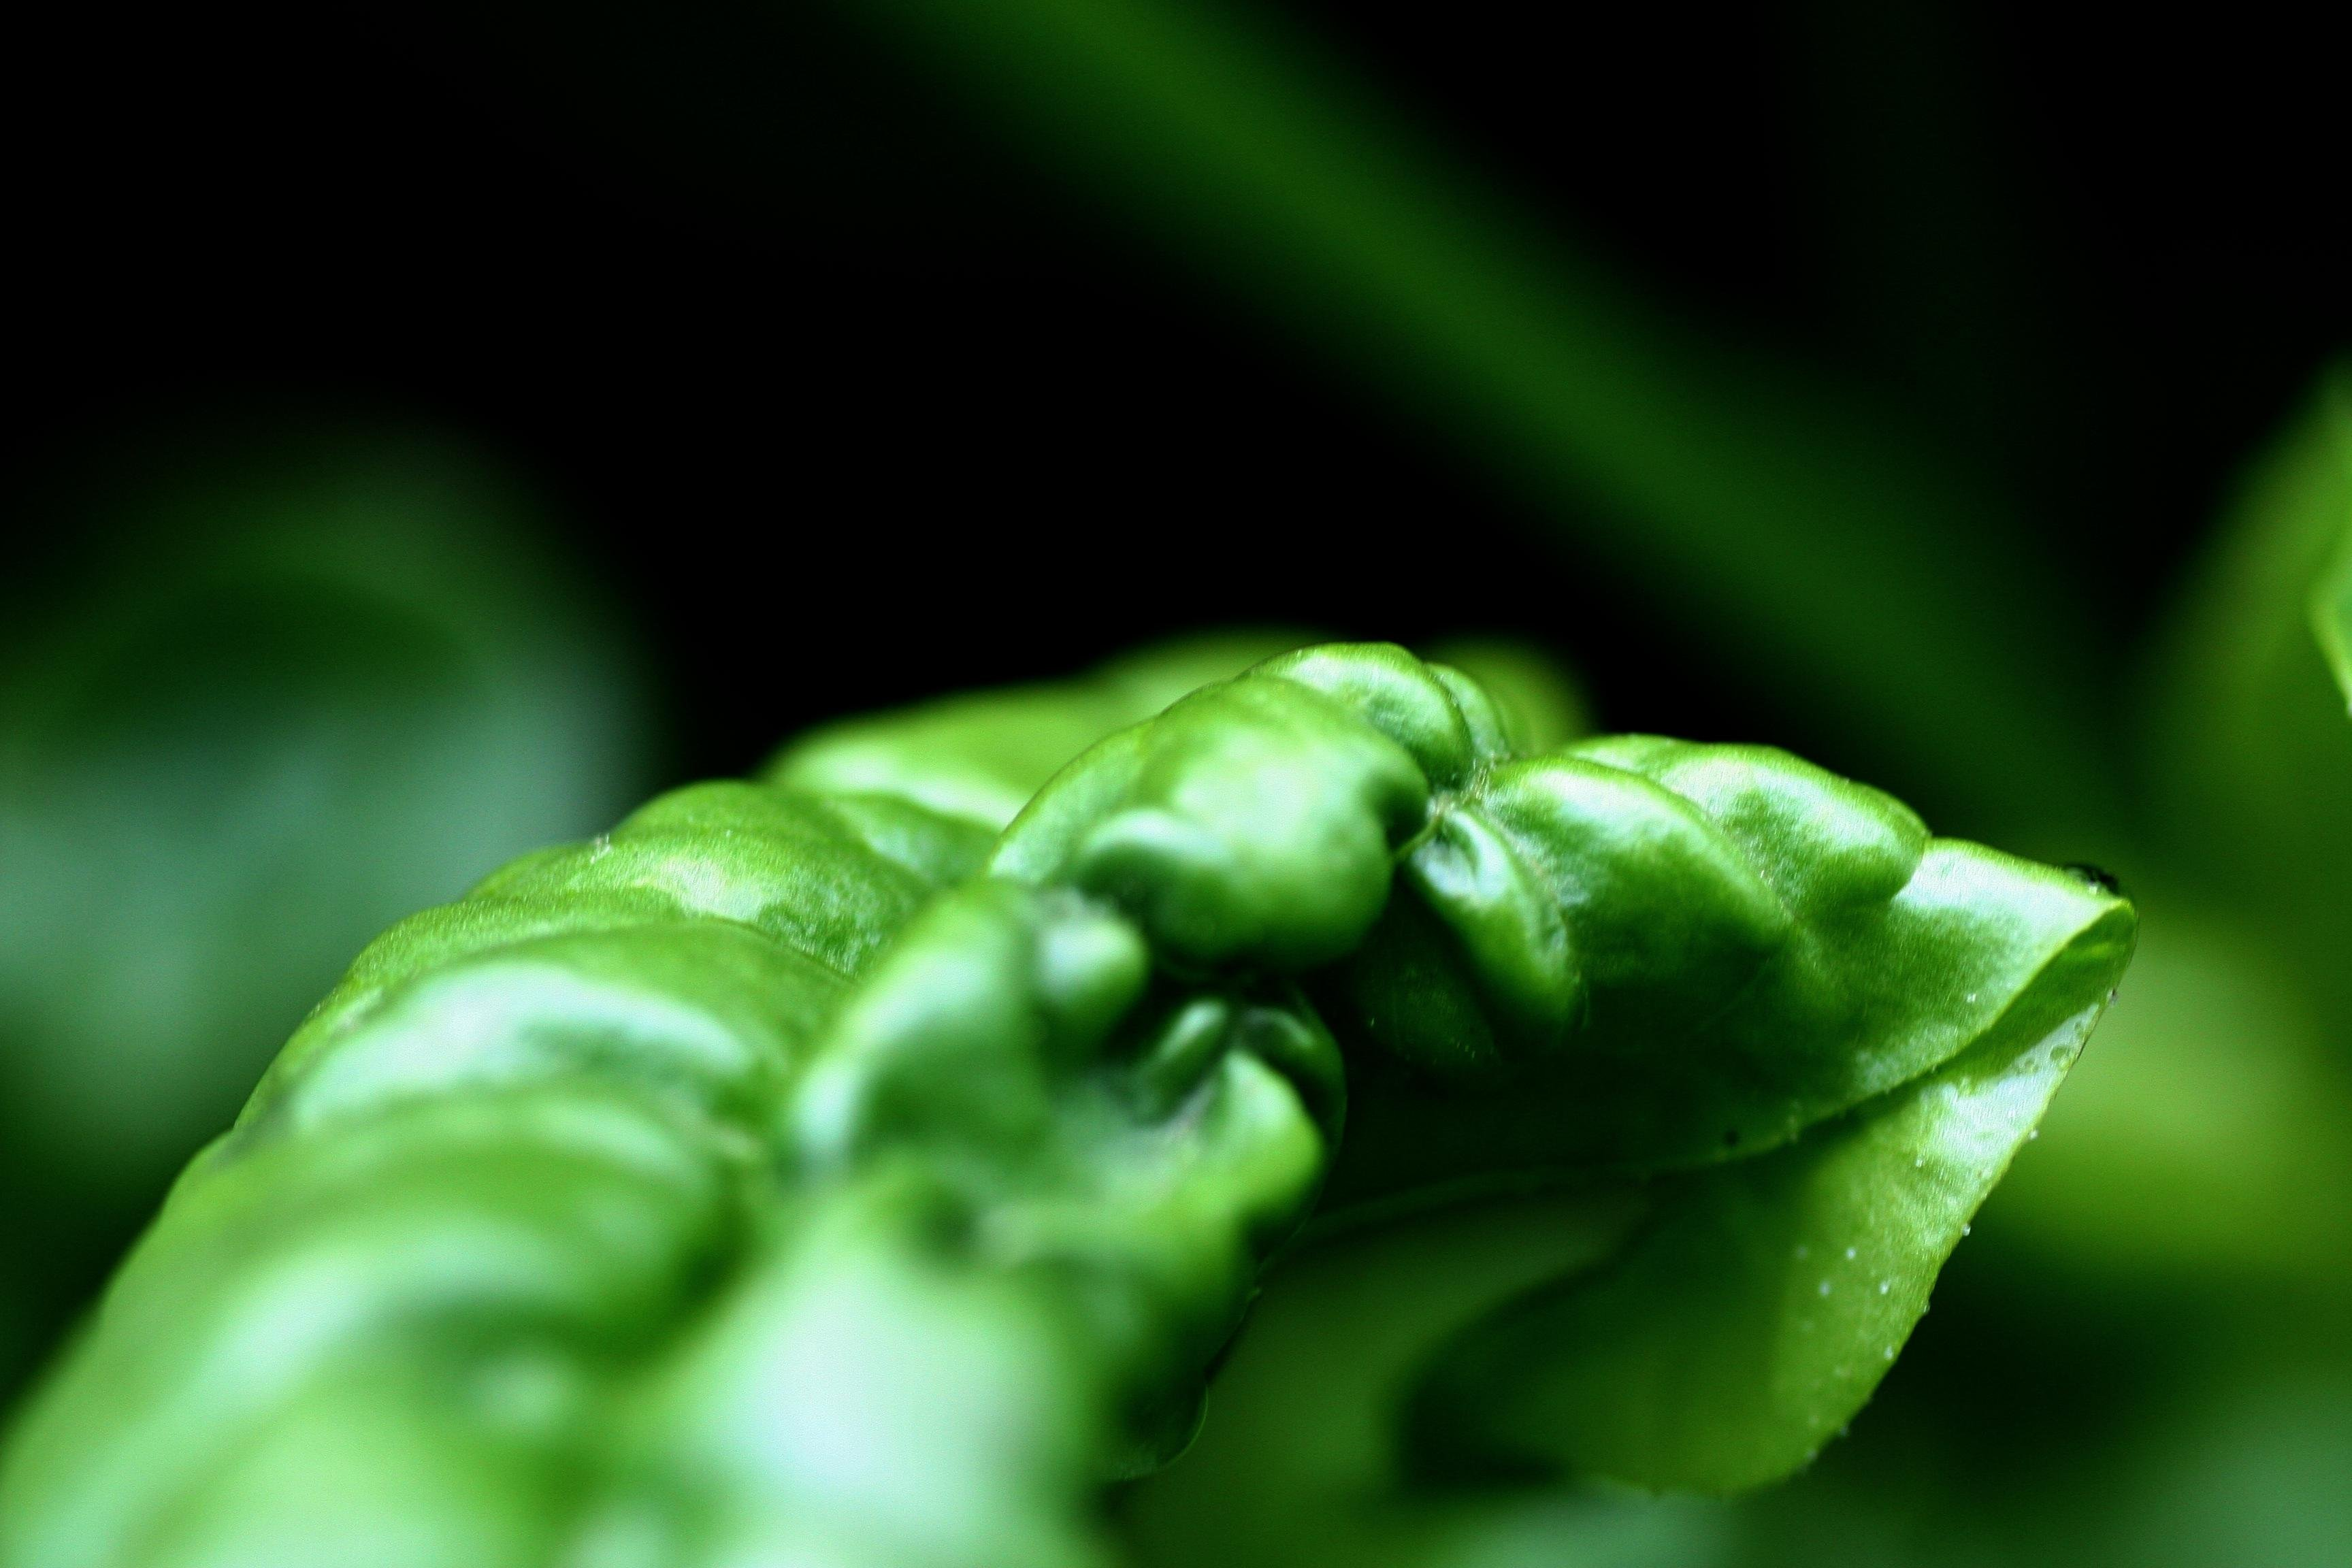
\includegraphics[width=\paperwidth,height=\paperheight]{spinach.jpg}
    \caption{Fresh Spinach}
\end{figure}
\restoregeometry
\clearpage

\section{Anne's Spinach Salad}
\begin{multicols*}{3}

\begin{quote}
    This recipe is from my Aunt Anne, who swears that she always used romaine lettuce instead of spinach.
\end{quote}

\begin{tabular}{r@{ }l}
    2 & eggs \\
\end{tabular}

Boil eggs, cool, shell and slice into rings.

\begin{tabular}{r@{ }l}
    10 & strips bacon \\
\end{tabular}

Separate strips onto aluminum foil in a baking sheet, and bake for 15 minutes at 425. Pat dry and chop into small pieces.

\begin{tabular}{r@{ }l}
    \sfrac{1}{2} & cup olive oil \\
    \sfrac{3}{4} & can anchovies in oil \\
               2 & tablespoons balsamic \\
               2 & tablespoons lemon juice \\
               1 & garlic clove \\
    \sfrac{1}{2} & teaspoon thyme \\
    \sfrac{1}{4} & teaspoon \\
                 & sugar \\
                 & oregano \\
                 & mustard powder \\
                 & onion salt \\
                 & paprika \\
\end{tabular}

Discard the oil in the can and use only the anchovies. Liquefy all  ingredients in a blender.

\begin{tabular}{r@{ }l}
    1 & package spinach \\
      & pre-sliced mushrooms \\
\end{tabular}

Combine eggs, bacon and dressing in a large mixing bowl.

\begin{quote}
The dressing can keep at least overnight.

To shell eggs easily, run under cold water, shaking pan to smash shells. The water will seep in. In 10 minutes, the shells will come off easily.

Leftover spinach can be saved, but be sure to reseal it in the original packaging, which is specially designed to breath. Spinach or lettuce saved in regular plastic will rot in a few days.

If you want to chop bacon very fine, freeze it for 10 minutes first.
\end{quote}

\end{multicols*}

\clearpage


\fullpageimage{couscous.jpg}{http://www.flickr.com/photos/stone-soup}

\section{Couscous Salad}
\begin{recipe}

\pre{
    Couscous has a tendency to clump together. Ideally, we want every kernel to be separate. Also, you want to serve the final salad as cold as possible. That means no lukewarm couscous.
}

\ingredients{
    1 & handful kosher salt \\
    3 & trays ice cubes \\
}

In one large metal bowl, combine ice, kosher salt, and enough water to cover the ice fully.

\ingredients{
    2 & boxes plain couscous \\
    1 & tablespoon butter \\
}

Follow the directions on the box to hydrate couscous. Immediately after the couscous is cooked, turn out into another metal bowl.

\columnbreak

\ingredients{
    \sfrac{1}{2} & cup Italian dressing \\
}

Mix the dressing into the couscous to help it separate. Fluff with a spatula, breaking up as many clumps as possible.

Place the metal bowl with the couscous into the bowl with the ice. Keep stirring every three minutes to break down the clumps.

\ingredients{
                6 & ounces feta cheese \\
                1 & orange bell pepper \\
                1 & yellow bell pepper \\
     \sfrac{1}{2} & large red onion \\
}

Dice the peppers and onion fine, and combine with feta cheese in the couscous bowl.

\ingredientsLeft{
    & Italian dressing \\
    & kosher salt \\
    & pepper \\
    & dried dill \\
}

Season to taste.

\columnbreak

\tip{
    The two large metal bowls with ice water is great for cooling just about anything quickly. It's kind of like a reverse double-boiler.
}

\tip{
    The boxed Couscous sold in the grocery store is actually pre-cooked, which is why it only takes a few minutes to hydrate. You can buy uncooked Couscous, which has larger grains and cooks like pasta.
}

\tip{
    When buying feta, I prefer the cryo-packed version with a little bit of juice sealed in. The free-standing feta in juice and the Saran-wrapped versions are dryer.
}

\end{recipe}

\section{Potato Salad}
\begin{recipe}

\pre{
    The key to this potato salad is cooking and cooling the potatoes completely, before 
    cutting them up, or stirring them. Otherwise, the potatoes start to break down and 
    muddy the salad. While they are hot, you want to both salt and season them with 
    vinegar (pickle juice). If you can cook the potatoes inside a fitted colander inside 
    a large pot, then they will bairly be distrubuted while cooking or cooling. 
}

\ingredients{
    3 & pounds medium or small yukon gold potatoes \\
    4 & quarts water \\
    & kosher salt \\    
    & pickle juice \\ 
}

Heavily salt water, put potatoes in, and bring to a boil. The water does not need to 
be at a boil before you put the potatoes in. Once boiling, reduce heat to a 
medium boil. Cook for 15 to 25 minutes, or until a knife easily pierces a potato. 

Drain potatoes using a colander. Place a colander with potatoes inside a large bowl. 
Pour (strained) pickle juice over the hot potatoes. Using another large bowl, move 
colander back and forth, and continue to pour the pickle juice over the potatoes every 
minute, until they stop steaming.

Leave potatoes out at room temperature to cool completely, before cutting them. 

\ingredients{
                2 & cups mayonnaise \\
                3 & celery stalks \\
                1 & small white onion \\
                1 & tablespoon celery seed \\
                2 & tablespoons dijon mustard \\
                3 & sprigs fresh dill \\
                  & fresh parsley \\
}

Dice celery, onion, dill and parsley fine. Whisk to combine with wet ingredients.
Season to taste with salt and pepper.

\ingredients{
      & paprika \\
}

Combine the potatoes and sauce, and top with paprika.

\end{recipe}


\fullpageimage{panzanella.jpg}{http://www.flickr.com/bonequinha\_sf/}

\section{Panzanella}
\begin{recipe}

\pre{
    When you make a salad with wet ingredients like tomatoes and cucumber, often times you get a pool of juice in the bottom of the bowl.

    This recipe, also known as Italian Bread Salad, soaks up that flavorful juice with toasted bread.

    The key is to let the salad rest for 10 minutes while the bread soaks up the juices.
}

\ingredients{
    1 & loaf rustic bread \\
    2 & tablespoons olive oil \\
}

Slice the bread into 1 inch cubes. Toss with olive oil and salt and place cubes on a rack on top of a rimmed baking sheet, and toast at 400\degree for 20 minutes, or until golden brown.

\ingredients{
    1 & pint cherry tomatoes \\
    1 & cucumber \\
      & salt \\
}

Slice cherry tomatoes in half. Peel cucumber, slice in quarters lengthwise and remove seeds with a spoon. Then slice cucumber sticks into rough dice.

Salt tomatoes and cucumbers, and let drain over a bowl for 20 minutes, reserving the liquid.

\ingredients{
                3 & tablespoons red wine vinegar \\
     \sfrac{1}{2} & cup olive oil \\
                1 & shallot \\
}

Whisk finely minced shallot with oil and vinegar, set aside.

\ingredients{
    3 & ounces feta cheese \\
      & fresh basil \\
      & salt \\
      & pepper \\
}

Toss bread cubes with tomatoes, cucumbers, dressing, feta and chopped basil. Toss to coat, adding reserved tomato liquid. Season with salt and pepper.

\end{recipe}


\fullpageimage{chickensalad.jpg}{http://www.flickr.com/photos/paqman/}

\section{Curried Chicken Salad}
\begin{recipe}

\pre{
    Store bought roasted chicken is also good. The slight barbeque flavor that remains after you remove the skin goes well with curry.

    Bone in, skin on chicken breast will give the meat more flavor.
}

\ingredients{
    2 & chicken breasts \\
      & salt \\
}

Salt chicken breasts, and let them rest for 1 hour. Roast in a 400\degree over until meat registers 165\degree, about 40 minutes.

Cool to room temperature, and shred with a fork.

\ingredients{
    2 & celery stalks \\
    2 & scallions \\
    2 & tablespoons cilantro \\
    1 & cup mayonnaise \\
    6 & tablespoon golden raisins \\
    2 & tablespoons lime juice \\
    2 & teaspoons curry power \\
    1 & tablespoon honey \\
      & salt \\
      & pepper \\
}

Chop celery, scallions and cilantro fine, and combine with other ingredients.

Let the mixture sit for 15 minutes before serving in sandwiches.

\subsection{Lettuce Wraps}

This can also be served in romaine lettuce leaves. In this case, I would  add chopped walnuts and sliced green grapes.

\end{recipe}


\section{Salad Dressings}
\begin{recipe}

\subsection{Phil's Famous}

\pre{
    My father used to make this dressing for salads and marinades at almost every family gathering, as well as once a week for regular dinners.
}

\ingredients{
    3 & tablespoons olive oil \\
    2 & tablespoons vinegar \\
    1 & tablespoon Grey Poupon \\
    1 & teaspoon oregano  \\
    1 & garlic clove \\
}

Combine ingredients in a small jar, and shake vigorously. The emulsion is stable for at least an hour.

\subsection{Lemon Vinaigrette}

\pre{
    This simple dressing is from Pam and Rick. I remember them serving it many times in Bar Harbor.
    It's great with just mixed greens, or with cucumber.
}

\ingredients{
    1 & garlic clove \\
}

Cut clove in half and rub the against the inside of a wooden salad bowl. Discard the clove.

\ingredients{
    3 & tablespoons olive oil \\
    2 & tablespoons lemon juice \\
    1 & teaspoon kosher salt \\
}

Combine ingredients in the bottom of the bowl, whisk to combine, and toss salad.

\subsection{Parmesan Peppercorn}

\ingredients{
    \sfrac{3}{4} & cup mayonnaise \\
    \sfrac{1}{4} & cup sour cream \\
               3 & tablespoons Parmesan \\
               2 & tablespoons milk \\
               2 & tablespoons vinegar \\
               1 & tablespoon black pepper \\
               1 & teaspoon garlic powder \\
               1 & teaspoon basil \\
}

Whisk together in a medium bowl, and refrigerate for at least an hour.

\end{recipe}


\chapter{Week Nights}

\section{Fleming's Macaroni and Cheese}
\begin{recipe}

\pre{
    This is the actual recipe for a favorite side-dish from Fleming's Steak House. The recipe was published on the web by their head chef.

    Finding smoked cheddar can be somewhat challenging, but it is critical to the dish.
}

\ingredients{
    1 & box cavatappi pasta \\
    2 & teaspoons salt \\
    1 & tablespoon veg oil \\
}

Bring one gallon of water to boil. Add 2 teaspoons salt and cook pasta very al-dente. Drain pasta and cool under cold running water. Toss drained pasta in oil and reserve.

\columnbreak

\ingredients{
    \sfrac{3}{4} & cup onion, small dice \\
               1 & stick unsalted butter \\
               3 & tablespoon flour \\
}

In a dutch oven, sauté onions over medium heat. Add flour and cook for one minute, but do not brown.

\ingredients{
    2 & cups heavy cream  \\
    3 & cups half and half \\
    2 & teaspoons kosher salt \\
    1 & teaspoon white pepper \\
}

Add cream, half and half, kosher salt and white pepper. Bring pot to a simmer. Cook until sauce is thick, about 5-6 minutes.

\ingredients{
    \sfrac{3}{4} & pound smoked cheddar \\
    \sfrac{1}{4} & pound cheddar cheese \\
}

Still in the dutch oven, blend grated cheese into sauce until melted. Add pasta.

\ingredients{
               1 & tablespoon veg oil \\
               1 & teaspoon chipotle powder \\
    \sfrac{3}{4} & cup panko bread crumbs \\
}

Sauté oil and chipotle powder over medium-high heat for 30 seconds. Remove from stove and stir in bread crumbs.

Sprinkle bread crumbs over the pasta and bake for 15-20 minutes at 350\degree.

Variation: add chunks of roasted broccoli.

\end{recipe}

\fullpageimage{macandcheese.jpg}{http://www.flickr.com/photos/kendallsentertaininglife/}



\section{Cream of Mushroom and Chicken}
\begin{recipe}

\pre{
    This is great for a cold week night, and it re-heats very well.

    Shredding the chicken versus cutting into pieces helps the texture.
}

\ingredients{
    2 & chicken breasts, skin on \\
}

Brown chicken on all sides in a dutch over over medium-high. Remove chicken, but leave the rendered fat.

Roast chicken in the oven for 12 more minutes at 450\degree, flipping once half way.

\ingredients{
    10 & ounces dried mushrooms \\
     1 & package fresh mushrooms \\
     3 & cloves garlic \\
}

Rehydrate fried mushrooms in water for 15 minutes. Sauté all mushrooms over medium heat in the chicken far for 10 minutes, and then add minced garlic.

\ingredients{
    1 & cup heavy cream \\
    1 & cup half and half \\
}

Combine in the dutch oven along with mushrooms, and return to medium heat.

After 10 minutes of simmering, blend using a stick blender (or standing blender) until very smooth.

\ingredients{
    1 & package frozen peas \\
    1 & red pepper \\
}

Shred chicken into small pieces and add to soup mixture, along with peppers and peas. Season to taste with salt and pepper.

\ingredients{
    1 & cup rice \\
    1 & package puff pastry \\
}

Start the rice, and follow package instructions to bake puff pastry. Most pastry needs to be brought to room temperature for 40 minutes.

Serve inside a puff pastry on top of rice.

\end{recipe}


\fullpageimage{steaktips.jpg}{http://www.flickr.com/photos/dongkwan}

\section{Steak Tips}
\begin{recipe}

\pre{
    Almost anything could be labeled as steak tips in the grocery store. I use a cut that comes as a two inch square, foot long piece of loose fibered meat, and which is labeled simply "Steak tips".
}

\ingredients{
    1 & large onion \\
    3 & tablespoons butter \\
      & kosher salt \\
}

Cut onion into rings, and salt. Melt butter over medium heat in a sauté pan. Add onions.

\ingredients{
    1 & pound sirloin steak tips \\
    1 & tablespoon butter \\
}

Pat meat dry with paper towels.

In a large deep frying pan, melt butter over medium heat. Increase heat to high and sear meat without moving it for three minutes a side.

Remove from heat, rest for 6 minutes and cut steak tips into 1\sfrac{1}{2} inch cubes.

\subsection{American Style}

\ingredients{
    1 & cup ketchup \\
    5 & tablespoons soy sauce \\
    1 & teaspoon malta \\
}

Whisk together wet ingredients in a small bowl. Combine with remaining ingredients in a small bowl.

Add sauce and steak tips into the large pan, spread out. Simmer on medium heat for 30 minutes, stirring every five minutes. The sauce will reduce and congeal, turning a darker brown.

Season with salt and pepper to taste.

\ingredients{
    1 & package egg noodles \\
      & water \\
    4 & tablespoons butter \\
}

Bring water to a boil, add egg noodles and cook until al dente. Drain, return to pot and stir until sticky. Incorporate butter until melted.

Serve steak tips and sauce on top of the noodles.

\subsection{Asian (Yen Tieu) Style}

\ingredients{
    \sfrac{1}{4} & cup fish sauce \\
    \sfrac{1}{4} & cup lime juice \\
    \sfrac{1}{4} & cup water \\
               3 & tablespoons sugar \\
               2 & garlic cloves \\
               1 & minced jalapeno \\
}

Combine sauce ingredients and serve over white rice.

\end{recipe}


\fullpageimage{burger.jpg}{http://www.flickr.com/photos/pointnshoot}

\section{Drive-Thru Burgers}
\begin{recipe}

\pre{
    The key to this recipe is to keep the patties loose, so the juices can bubble up through the nooks and crannies as they cook. This makes them both crisp and juicy.

    The rolls should be sautéd before cooking the burgers, so that the burgers are still crispy when served.

    Instead of crowding all the burgers into one pan, do them in batches so that they will crisp up instead of steaming.
}

\ingredients{
    2 & parts sirloin tips \\
    1 & part beef short ribs \\
      & kosher salt \\
}

Cut both meats into one-inch cubes, spread uncrowded on plates and freeze for 15-20 minutes.

\ingredients{
    & unsalted butter \\
    & Kaiser rolls \\
}

For each roll, melt one tablespoon of butter in a sauté pan over medium heat, and fry both roll halves face down until golden brown, about 3 minutes.

Remove meat from freezer.

Working in batches with a 2:1 ratio of steak tip to short rib, pulse in a food processor to a coarse ground meat consistency (About 10 one-second pulses).

Spread ground meat onto baking sheets and hand-mold into loose, thin burgers. Season liberally with salt and pepper.

\ingredients{
    & slices American cheese \\
    & vegetable oil \\
}

Add one tablespoon oil to a large sauté pan over high heat, along with the burgers. Don't move the burgers at all for at least three minutes, or until the juices are bubbling through the raw layer on top.

Flip burgers. Add one slice of cheese to each, and cook for another two minutes without flipping.

\tip{
    Best served with thinly sliced onions, and not much else.
}

\subsection{"Secret Sauce"}

\pre{
    This is the identical to Big-Mac sauce.
}

\ingredients{
    1 & part mayonnaise \\
    1 & part ketchup \\
    1 & teaspoon sweet relish \\
      & fresh pepper \\
}

Whisk ingredients together in a small bowl, add pepper and sweet relish to taste.

\end{recipe}


\section{Taco Night}
\begin{recipe}

\pre{
    With ground beef, you want to nearly burn it to develop some flavor.
}

\ingredients{
    1 & pound ground beef \\
}

Fry in a cast iron pan over medium-high heat. Don't flip it at all for at least 10 minutes.

\ingredients{
               2 & tablespoons chili powder \\
               1 & teaspoon cumin  \\
               1 & teaspoon coriander  \\
    \sfrac{1}{2} & teaspoon oregano  \\
    \sfrac{1}{4} & teaspoon cayenne \\
    \sfrac{1}{4} & cup chicken broth \\
               1 & can Adobe sauce, chilies removed \\
}

Dump the spice mixture on top. Smother in chicken broth and Adobe sauce, and stir to combine.

Cook for 10 minutes.

\ingredients{
    1 & cup white rice \\
    1 & tablespoon olive oil \\
    2 & garlic cloves \\
    2 & cups chicken broth \\
    3 & tablespoons chopped parsley \\
}

Brown rice with oil. Add smashed garlic clove and chicken broth and bring to simmer.
Reduce to low, cover with a dish towel between the lid and the pot and
cook for 25 minutes.

\ingredients{
    8 & six inch corn tortillas \\
    2 & cups vegetable oil \\
}

Heat the vegetable oil over medium heat in a frying pan just big enough to fit one tortilla.

Fry each tortilla for 30 seconds per side. Remove to a paper towel lined cooling rack.

Blacken flour tortillas directly over the gas flames.

\ingredients{
    & sour cream \\
  2 & limes \\
  1 & tablespoon hot sauce \\
}

Mix together.

\ingredientsLeft{
    & Monterey Jack cheese \\
    & onion \\
    & refried beans \\
    & lettuce \\
}

Wrap corn tortillas in flour tortilla shells and serve with various accoutrements.

\end{recipe}


\fullpageimage{buffalo.png}{}

\section{Buffalo Chicken Burritos}
\begin{recipe}

\pre{
    If the oil is hot enough, it will bubble furiously when you add the chicken.
}

\ingredients{
    \sfrac{1}{2} & cup blue cheese \\
    \sfrac{3}{4} & cup mayonnaise \\
    \sfrac{1}{4} & cup sour cream  \\
               2 & tablespoons milk \\
}

Whisk to combine in a small bowl, and refrigerate for at least an hour for the flavors to come together.

\ingredients{
    2 & pounds chicken tenders \\
    2 & cups flour \\
    2 & eggs \\
    1 & cup panko bread crumbs \\
}

Beat the eggs and put then in a shallow dish. Place the bread crumbs in another shallow dish. Place the flour in a small container with a lid, large enough to hold a few tenders.

Coat each piece of chicken with flour, and shake off the excess. Dip each side into the egg mixture, then place in the bread crumb container.

When you have three tenders in the bread crumbs, put the lid on a shake to coat each piece.

Remove chicken pieces to a wire rack, keeping as many of the bread crumbs adhered as possible.

Let the chicken rest for 20 minutes on the wire rack.

\ingredients{
    ½ & cup rice \\
    1 & cup water \\
    2 & tablespoons butter \\
}

Bring the water to a boil, then add the rice. When the water starts to boil again, reduce heat to low and put on the liquid.

\ingredients{
    1 & small container of crisco \\
}

Add the Crisco to a heavy 12 inch frying pan over medium heat. When the oil reaches 350 degrees, add the first piece of chicken.

Cook the chicken until it's fully browned, about three minutes a side. If it browns too quickly, don't be afraid to flip or remove it, and finish it in a 350 degree oven for more even cooking.

Let the cooked chicken rest for 15 minutes, then chop it roughly into one inch pieces.

\ingredients{
    12 & inch flour tortillas \\
     2 & stalks celery \\
}

Heat up the tortillas for 60 seconds in the microwave. Once at a time, roll each tortilla with rice, chicken, blue cheese sauce and celery roughly chopped.

\end{recipe}


\fullpageimage{dandannoodles.jpg}{}

\section{Dan Dan Noodles}
\begin{recipe}

\pre{
    If you have some of the Chinese condiments already, you can make this dish for under 10 dollars.

    The chili sauce I like has a rooster on the label. It's in the Chinese section. You want the white label, not the gold one.
}

\ingredients{
    \sfrac{1}{3} & cup peanut butter \\
               2 & garlic cloves \\
               2 & tablespoons fresh ginger \\
               2 & tablespoons brown sugar \\
               1 & tablespoon sesame oil \\
               1 & tablespoon black vinegar \\
               1 & tablespoon garlic chili sauce \\
}

Pulse in a food processor until smooth.

\ingredients{
    \sfrac{1}{4} & cup chicken broth \\
}

Slowly add the broth to the running food processor to emulsify.

\ingredients{
    4 & packages of Ramen noodles \\
}

Throw away the flavor packets.

Boil in water for 90 seconds. Drain in a colander, and quickly remove to a large bowl.

Add the sauce to the bowl, and mix to coat the noodles.

\ingredients{
    \sfrac{1}{2} & cup roasted unsalted peanuts \\
               3 & scallions \\
}

Chop the scallions fine. Pulse the peanuts just a few times in the dirty food processor.

Plate the noodles and top with scallions, peanuts and more chili sauce.

\end{recipe}


\fullpageimage{bakedziti.jpg}{http://www.flickr.com/photos/benreichelt}

\section{Baked Ziti}
\begin{recipe}

\pre{
    I usually make this with two dutch ovens, but you could also use a dutch oven and a sauté pan.
}

\ingredients{
    1 & pound rigatoni \\
}

Boil in salted water for five minutes less than the box directions. It will continue to cook in the oven.

\ingredients{
    28 & ounce tomato sauce \\
    14 & ounces diced tomatoes \\
     1 &  small onion \\
     5 &  cloves garlic \\
     3 &  tablespoons fresh basil \\
     2 &  teaspoons sugar \\
     1 &  teaspoon dried Oregano \\
}

Dice onions and sauté with olive oil in a small dutch oven until soft. Add minced garlic and cook until straw colored.

Add tomatoes, sauce, sugar and Oregano and simmer for 15 minutes. Stir in chiffonade basil and season with salt and pepper.

\ingredients{
    24 & ounces cottage cheese \\
     1 &  cup heavy cream \\
     1 &  cup grated Parmesan \\
     2 &  eggs \\
     1 &  tablespoon corn starch \\
     1 &  tablespoon hot sauce \\
}

Whisk cream and cornstarch in a dutch oven, and simmer over medium for two minutes.

Add cottage cheese, Parmesan, hot sauce and eggs, and mix with a wooden spoon. Add two cups of the tomato sauce and combine.

Add drained pasta, and toss to coat.

\columnbreak

\ingredients{
    1 & pound mozzarella \\
}

Cut mozzarella into \sfrac{1}{4} inch cubes, and add half to the pasta.

Cover the pasta with the remaining tomato sauce, and then the remaining mozzarella.

Bake for 30 minutes covered at 375\degree, then another 30 minutes uncovered. If it's not browned, put it under the broiler for 5 minutes.

Cool for 20 minutes, and serve.

\end{recipe}

\section{Broccoli Sausage Orecchiette}
\begin{recipe}

\pre{
    This recipe relies on a good parmesan cheese, and a good olive oil. Don't
    skimp on the full half cup of oil. Romano is good, too.
}

\ingredients{
               3 & large Italian sausages, or one package of sausage mix \\
    \sfrac{1}{2} & cup olive oil \\
                 & red pepper flake \\
}

Pre-heat oven to 550\degree{}.

If using sausage, remove casing from sausages with a sharp knife.

Shallow fry in olive oil in a dutch oven over medium-high heat until
browned. Removed with a slotted spoon and process in a food processor for 3
short bursts. This will break up the sausage into the right sized pieces.
Return to pan and brown for another 10 minutes on medium heat.

Add red pepper flakes (even if using spicy sausage).
Drain sausage, reserving the oil.

\ingredients{
    1 & head broccoli \\
      & more olive oil \\
      & red pepper flakes \\
      & salt \\
      & pepper \\
}

Slice broccoli stalk into thin disks about 1/8 inch.

Toss in the reserved sausage oil in the now empty dutch oven. Turn out into a
foiled baking sheet, and place under the broiler until lightly blackened.

\ingredients{
    1 & box Orecchiette pasta \\
}

Boil paste until al dente, as per box instructions. Drain, reserving a bowl
of the water.

Add the sausage and broccoli to the pasta. Toss to combine.
Season with salt, pepper.

\ingredients{
    6 & ounces parmesan \\
}

Grate the parmesan on the finest setting. When the paste has cooled for 5
minutes, toss with cheese and reserved pasta liquid. The goal is to create a
cheese sauce.

\tip {
    Great with Sriracha.
}

\end{recipe}


\chapter{Weekends}

\section{Perfect Omelet}
\begin{recipe}

\pre{
    Eggs want to be handled and heated as little as possible for maximum tenderness. That is why I start with room temperature eggs.

    Developing a curd by swirling the eggs for a few seconds after they have hit the pan adds texture.

    Many cooks keep a separate omelet pan. It's not strictly necessary, but I prefer a cast-iron pan with very low sides.

    Finally, don't add too much filling. Keep the filling to a minimum, and pre-cook any filling except cheese.
}

\columnbreak

\ingredients{
    1 & bell pepper \\
    1 & small onion \\
}

Dice fine, and pre-cook over medium heat until the onions start to brown. Remove from heat and reserve.

\ingredients{
    3 & eggs, room temperature \\
    1 & teaspoon dried dill \\
      & pinch kosher salt \\
}

Crack eggs into a medium bowl, salt, and whisk lightly with dill.

\ingredients{
    1 & tablespoon butter \\
}

Heat the pan over medium heat for five minutes. Coat with butter, removing excess, and wait a few minutes until the butter stops bubbling.

Pour egg mixture into the pan, and immediately stir with a spatula. In just a few seconds, a few large curds will have formed. Shake the pan to redistribute raw egg into any gaps.

\ingredients{
    1 & ounce feta cheese \\
}

Top two thirds of the omelet with cheese, pepper and onion. Cook until the raw egg has firmed up everywhere, and bubbles have started to form.

Run the tip of a spatula around the rim of the omelet, separating it from the pan.

Give the pan a firm shake, dislodging the omelet from the pan surface.

Using the spatula, flip the third of the omelet with no filling onto itself.

Shaking the pan, slide the folder end of the omelet onto a plate, and flip the remaining part over the top.

\end{recipe}

\fullpageimage{omelet.jpg}{http://www.flickr.com/photos/stone-soup}


\section{Pancakes}
\begin{recipe}

\pre{
    I used to make pancakes from scratch, using either buttermilk or buttermilk powder. 
    But it turns out that even basic pancake mix like Bisquick has all the basic ingredients 
    I was using, and nothing more. 
}

\ingredients{
               2 & cups pancake mix \\
               2 & teaspoons sugar \\
}

Whisk in a large bowl to combine.

\ingredients{
    2 & eggs \\
    1 & cup of whole milk \\
    1 & dash of vanilla extract \\
}

Beat eggs in a separate bowl, and add milk and vanilla extract. 

Combine wet and dry ingredients, stir well with a spatula to combine. Make sure to 
get any of the dry bits. 

\ingredients{
    & vegetable oil \\
}

Preheat an electric griddle to 375\degree{}. You can also use the largest frying pan you have over medium-low heat.

For each batch of pancakes, add 3 tablespoons of vegetable oil to the pan.

You want a pool covering the entire surface.

Pour \sfrac{1}{4} cup of the batter onto an empty spot on the pan, and repeat until the pan is full.

After about 80 seconds, flip them, and cook for 80 seconds.

Transfer the pancakes to a wire rack on a sheet pan while the others finish.

\end{recipe}


\fullpageimage{pizza.jpg}{http://www.flickr.com/photos/maveric2003}

\section{Deep Dish Pizza}
\begin{recipe}

\pre{
    Instead of a pizza stone, we use a large square brick we bought at Home Depot for three dollars. It's not strictly necessary; the crust browns pretty well without a stone.
}

\ingredients{
    3\sfrac{1}{4} & cups flour \\
     \sfrac{1}{2} & cup cornmeal \\
                2 & teaspoons salt \\
                2 & teaspoons sugar \\
                1 &  packet yeast \\
    1\sfrac{1}{4} & cups warm water \\
                3 & tablespoons melter butter \\
}

Mix dry ingredients in stand mixer. Add water and melted butter, and mix on medium-high for 5 minutes.

Empty the dough into an oiled bowl, turn to coat surface, and let rise for 1 hour.

Empty dough onto the counter top, and use a rolling pin to flatten into a 12 by 15 inch rectangle. Slather with softened butter, and roll into a cylinder, like a jelly roll.

Flatten the cylinder into an 18 by 4 inch rectangle with the rolling pin. Cut in half, and fold the ends of each half in on itself, like a letter.

Shape each half into a rough ball, and place back into the oiled bowl for 1 hour to rise.

Shape the dough to cover the pan surface, as well as one inch up the sides. If the dough resist shaping, let sit for 10 minutes and try again.

\ingredients{
    28 & ounces crushed tomatoes \\
     1 & onion \\
     1 & tablespoon olive oil \\
     1 & tablespoon tomato paste \\
     1 & clove garlic \\
       & red pepper flakes \\
       & kosher salt \\
}

In a dutch oven over medium heat, brown shredded onion with olive oil. Add tomato paste, garlic and red pepper flakes, and cook for 30 seconds. Add crushed tomatoes simmer for 15 minutes. Salt to taste.

\ingredients{
    \sfrac{3}{4} & pound mozzarella cheese \\
               3 & Italian sausages \\
}

Taking the stuffing out of the sausages, press quarter sized pieces directly into the dough. Top will cheese, and finally tomato sauce. Optionally, top with a sprinkling of Parmesan.

Bake for 25 minutes at 350. Don't worry, the sausage will be done. Rest for 15 full minutes and then remove from baking dish before slicing and serving.

\tip{
    Variation: skip the sauce, and top with chopped bacon, caramelized onions and thyme. Onions can be caramelized by sautéing on low for an hour with 3 tablespoons of butter, and a sprinkle of salt and sugar.
}

\end{recipe}

\section{Lasagna}

\begin{recipe}

\pre {
    This is a kid-friendly lasagna, no ricotta or bechamel sauce. This will be even better 
    if you make it ahead of time and reheat it in the oven. Meatloaf mix (or raw meatloaf to be cooked) is sold 
    at many butcher counters; it's a mix of beef, veal and pork. You can also substitute 80/20 beef.
    One box of noodles is plenty for a medium lasagna. This will seem like a lot of sauce, but the lasagna 
    will absorb it. Total cooking time is 4.5 hours. 
}

\ingredients{
    42 & ounces chuncky tomato sauce (1 large cans, 1 small can) \\
    28 & ounces San Marzano whole tomatoes in sauce (1 can) \\    
     1\sfrac{1}{2} & lbs meatloaf mix \\
     1 &  cup whole milk \\
     2 &  cloves garlic \\
     1 &  tablespoon tomato paste \\
     1 &  tablespoon red pepper flakes \\
     1 &  large onion \\
}

Chop onion fine, and sauté in oil until just starting to brown. Add garlic and tomato paste and cook for 3 minutes.
Add meat and milk and bring to simmer. Add canned tomatoes, crushing the whole tomatoes with your hands. 
Simmer uncovered on the lowest heat for 2 hours.

\ingredients{
     1 & box regular Lasagna noodles \\
     2 & lbs block whole milk mozzarella, cubed \\
}

Boil noodles for just 4 minutes, or 4 minutes less than the cooking time. The idea is that they will finish in the oven,
and absorb the sauce. Drain noodles, and separate out on clean kitchen towels or baking sheets, so they do not stick together.

Pour a large ladle of sauce in the bottom of a smaller 9x13 baking dish, and spread it out.

Lay down a layer of six noodles, followed by a layer of cubed mozzarella, and a layer of sauce.

Repeat with a second layer. Don't use more than six noodles for the top layer, or it could buckle. 

\ingredients{
     2 & ounces Parmesan cheese \\
     1 & tablespoons garlic powder \\
}

Top with a final layer of noodles with enough tomato sauce so that there are no dry spots, more mozzarella, and the grated Parmesan.

Bake at 375\degree{} for 40 minutes.

Remove from the oven, and let cool for 60 minutes before serving.

\end{recipe}

\section{Red Chile Chicken Enchiladas}
\begin{recipe}

\ingredients{
    1 & tablespoon veg oil \\
    1 & onion \\
}

Chop onion fine, and sauté in a Dutch oven over medium heat until just starting to brown.

\ingredients{
    3 & garlic cloves \\
    3 & tablespoons chili \\
    2 & teaspoons coriander \\
    2 & teaspoons cumin \\
    2 & teaspoons sugar \\
    1 & teaspoon oregano \\
    1 & teaspoon kosher salt \\
}

Mix ingredients, sauté for 30 seconds on high, then add to onions. Stir for 30 seconds.

\ingredients{
    2 & chicken breasts \\
}

Remove excess fat, and cut into \sfrac{1}{4} inch strips. Add to onions and spices, and stir until coated.

\ingredients{
    1\sfrac{1}{4} & cup tomato sauce \\
    1\sfrac{1}{4} & ounces heavy cream \\
    3\sfrac{1}{2} & ounces chipotle (in adobe sauce) \\
                1 & tablespoon lime juice \\
}

Add liquids, and simmer for 10 minutes. Pour mixture through a strainer, extracting as much sauce as possible. Reserve sauce and solids.

Chill the chicken for 10 minutes in the freezer.

Season red sauce to taste with salt, pepper and lime juice. Simmer for 10 more minutes.

\ingredients{
    \sfrac{3}{4} & pounds jack cheese \\
    \sfrac{1}{2} & pounds mild cheddar \\
               1 & cup fresh cilantro \\
              12 & ounces pickled jalapeños \\
}

Chop jalapeños and cilantro fine. Grate cheese, and combine all ingredients in a mixing bowl, along with the solids from the sauce. Combine with chicken.

\ingredients{
    10 & ten inch flour tortillas \\
}

Microwave tortillas for a minute to soften. Coat the bottom of a 9x13 baking dish with the red sauce.

One at a time, dip a tortilla in the sauce, fill with chicken and cheese mixture, roll up and place in the baking dish. Cover the dish with red sauce. There should be no dry tortilla.

Top with more cheese and bake uncovered at 375\degree{} for 25 minutes. Rest for 10 minutes before serving.

Serve with sour cream and lime wedges. Pairs well with Spanish rice and refried beans.

\end{recipe}


\listoffigures

\end{document}

short columns - see chicken salad
special column case on salad dressings
some ingredients don't wrap - see buffalo/dandan
some space between paraphraches
back page
look for three digit words - add degrees
